\chapter{Debating Same-Sex Marriage}

These notes follow Michael Sandel's twelfth Justice lecture closely in its order, pressure points, and argumentative rhythm. Prepared for the LazyLearn track and curated by LazyingArt LLC with Video2Book, they begin where the previous lecture ended: with the narrative conception of the self, the claim that obligations of solidarity are real, and the harder question of what happens when those ideas meet disputes about justice. The lecture's central burden is to show, first, that arguments about justice cannot finally be detached from arguments about the good, and second, that once this is admitted we still have a way of reasoning together.

\section{Narrative Self, Solidarity, and the Segregationist Challenge}

Sandel does not begin with a new topic. He resumes an unresolved difficulty from the previous meeting. We had been testing the narrative conception of the self, a conception according to which some obligations claim us not because we chose them, consented to them, or contracted into them, but because we stand within histories, memberships, and relations that help constitute who we are. In classroom discussion, loyalty, patriotism, and solidarity had acquired genuine intuitive force.

The pressure point is immediate. If obligations of membership are real, are they nevertheless always subordinate to duties owed to human beings as such? Sandel formulates the difficulty in a way we can summarize schematically as
\begin{equation}
\text{obligations of membership}
\stackrel{?}{<}
\text{duties owed to human beings as such}.
\end{equation}
This is not yet a conclusion. It is the opening problem.

What makes the problem urgent is the counterexample from the earlier film of southern segregationists. They too spoke in the language of history, identity, inheritance, and ``our way of life.'' If the narrative conception gives moral standing to loyalty and inherited attachment, does it also lend dignity to unjust traditions merely because they are someone's tradition?

\subsection{Question \& Answer}

\paragraph{Question.} Is the segregationist case a decisive objection to the narrative conception of the self?

\paragraph{Answer.} Not yet. The case shows that appeals to history and membership do not justify themselves simply by being inherited. But that is different from showing that no obligations of solidarity exist. The objection forces a further question: what account of justice allows us to distinguish legitimate solidarities from corrupt ones? That question will govern the rest of the lecture.

Sandel then states the day's program in two steps. First, he wants to defend the narrative conception of the person against the voluntarist conception associated with Kant and Rawls. Second, he wants to show that if obligations of solidarity are real, arguments about justice cannot after all be detached from questions of the good.

\section{Universal Duty, Friendship, and the Montesquieu Test}

The challenge to solidarity comes from a morally serious source. Sandel grants the appeal of the Kantian and Rawlsian picture: it is powerful, liberating, and universal in aspiration. It aims to treat persons as persons, without prejudice or discrimination. From this point of view it is tempting to say that even if obligations of membership exist, they must always be subordinate to universal duties.

Once we press that claim, however, it begins to transform the moral world. Sandel's question is not merely whether such universalism is noble, but what it would make of friendship, loyalty, and partial attachment. The line of pressure can be written as
\begin{align}
\text{universal loyalties always take precedence}
&\Longrightarrow
\text{friends/strangers distinction should be overcome},\\
\text{special concern for friends}
&=
\text{a kind of prejudice?},\\
\text{perfect virtue}
&\Longrightarrow
\text{no friends}.
\end{align}
The last line comes from Montesquieu's unsettling formulation: if men were perfectly virtuous, they would not have friends. A perfectly universalized moral imagination would leave us with no privileged attachments, only an equal readiness to come to the aid of anyone at all.

\subsection{Question \& Answer}

\paragraph{Question.} If universal human concern always takes precedence, what becomes of friendship?

\paragraph{Answer.} Friendship becomes morally residual, even suspect. It starts to look like a remnant of partiality that a better moral self would overcome. Sandel's answer is that this picture misses something essential. The deeper problem is not merely that such a world would be unrealistic; it is that it would scarcely be recognizable as a human world. We ordinarily learn to love humanity not in the abstract but through its particular expressions.

This is the first local payoff of the lecture. Smaller solidarities are not defended simply as unfortunate necessities. They are defended as part of the texture of a human moral life. Sandel is careful here: these are not knock-down arguments. Moral philosophy rarely offers those. But they are serious considerations, and they tell against the idea that universal concern can simply replace every special attachment.

\section{Two Ways Justice Can Be Tied to the Good}

Suppose, then, that the narrative conception and obligations of solidarity have some force. Sandel's next move is to test them by their consequences for justice. Here the segregationist difficulty returns in a sharper form. Are we forced to say that justice means whatever a given community, at a given time, says it means?

\begin{definition}
Sandel distinguishes two ways in which justice may be tied to the good. In the first, relativist way, justice is defined by the values or shared understandings that happen to prevail in a community. In the second, non-relativist way, justice depends on the moral worth of the ends that rights and institutions serve.
\end{definition}

A useful schematic summary is
\begin{equation}
\text{justice tied to the good}
=
\text{relativist way}
\;\;\text{or}\;\;
\text{non-relativist way}.
\end{equation}
The first route is formulated by Sandel as
\begin{align}
\text{relativist justice}
&=
\text{fidelity to the shared understandings of a tradition},\\
\text{relativist justice}
&\Longrightarrow
\text{justice as creature of convention}.
\end{align}
This is precisely what Sandel rejects. If justice is wholly conventional, it loses its critical character. It gives us no resources for criticizing the segregationists when they invoke their inherited way of life.

The second route keeps justice tied to the good without surrendering it to convention:
\begin{align}
\text{non-relativist justice}
&=
\text{rights justified by the moral worth of the ends they serve},\\
\text{case for recognizing a right}
&\Longrightarrow
\text{showing that it honors or advances an important human good}.
\end{align}
This is the route Sandel wants to defend. It is not communitarian in the crude sense of simply ratifying whatever a group happens to affirm. It is an attempt to say that questions of rights and justice require judgments about what is worthy of honor, protection, and recognition.

\subsection{Question \& Answer}

\paragraph{Question.} Does tying justice to the good make justice a creature of convention?

\paragraph{Answer.} Only on the relativist version. Sandel's point is that there is another possibility. We may tie justice to the good by asking what ends are genuinely worth serving. That move allows justice to remain critical rather than merely descriptive.

At this point the lecture reaches a new threshold. If justice is tied to the good in this non-relativist way, then how can we reason about the good in a pluralist society? Sandel does not answer this immediately. Instead he backs up to an easier question.

\section{Same-Sex Marriage as the Test Case}

Before asking whether we can reason about the good, Sandel asks whether such reasoning is unavoidable in the first place. His answer is yes, and same-sex marriage is introduced as the most revealing test. The issue implicates deeply contested moral and religious questions, and so it creates a powerful incentive to seek a neutral conception of rights that would avoid any public judgment about the moral status of homosexuality or the proper end of marriage.

The general claim can be put compactly as
\begin{equation}
\text{arguments about justice}
\not\!\!\perp
\text{questions of the good}.
\end{equation}
And the specific test becomes
\begin{equation}
\text{same-sex marriage decision}
\stackrel{?}{\Longrightarrow}
\text{a judgment about homosexuality and the telos of marriage}.
\end{equation}

\subsection{Question \& Answer}

\paragraph{Question.} Can we decide same-sex marriage without deciding the moral status of homosexuality and the telos of marriage?

\paragraph{Answer.} This is the question Sandel sets before the class. At the moment it is still open. The point of the classroom exchange is to see whether a neutral answer can survive sustained examination.

Mark and Ryan begin with a teleological argument. On this account, sex has a twofold purpose, procreative and unifying, and marriage as a social institution exists to honor and give expression to that purpose:
\begin{align}
\text{telos of sex}
&=
\text{procreation} + \text{union},\\
\text{purpose of marriage}
&=
\text{to honor and give expression to that telos}.
\end{align}
Ryan adds an important refinement. Homosexual conduct, on this view, need not be criminalized in order for the state to withhold marriage. The issue is not simply prohibition. It is whether the state should confer recognition and encouragement.

Hannah presses the first strong objection. If procreation is the defining telos of marriage, what do we say about infertile couples, older couples, or couples who cannot in fact have children? Sandel forces her to turn this from a personal challenge into a general argument.

\paragraph{Worked inference.}
\begin{align}
\text{if } \text{marriage} = \text{procreation only}
&\Longrightarrow
\text{infertile couples may not marry},\\
\text{but infertile couples may marry}
&\Longrightarrow
\text{procreation is not the sole telos of marriage}.
\end{align}
This does not by itself settle the same-sex-marriage question. But it blocks the simplest form of the procreative argument.

Steve then introduces the most important distinction of the classroom exchange, and Sandel explicitly calls it a good argument:
\begin{equation}
\text{moral permissibility of a practice}
\neq
\text{its fit with the honor or recognition of marriage}.
\end{equation}
This is a decisive structural clarification. One question asks whether a practice is morally permissible. Another asks whether a practice fits an institution to which the state attaches public honor and recognition. Once those are separated, the debate is no longer merely about private conduct. It is about the meaning of the institution.

\subsection{Question \& Answer}

\paragraph{Question.} Is there a difference between judging a practice morally and deciding whether the state should honor it as marriage?

\paragraph{Answer.} Yes. Sandel treats this as the crucial distinction that reorganizes the debate. One may, in principle, separate the morality of a practice from the public meaning of an institution. But once one does so, the issue becomes sharper rather than easier: what exactly is marriage, and what kind of union is it meant to honor?

That question leads to two neutrality-based responses. Victoria argues that the state should recognize civil union while refraining from deciding the telos of marriage itself. Cezanne goes further and says that if neutrality is really the point, the state should get out of recognizing marriages altogether. Sandel then states the chapter's central puzzle: unless we embrace the no-state-recognition option, can we decide same-sex marriage without taking a stand on the underlying moral and religious controversy over marriage?

\section{Reset, Goodridge, and the Failure of Pure Neutrality}

Here the lecture passes through a real seam. Sandel briefly steps back into the end-of-course register and reminds the audience that philosophy works by making the familiar strange. Only after that pause does he restart the argument at a higher level of abstraction: two remaining questions must be answered. Is it unavoidable to take up questions of the good when thinking about justice? And is it possible to reason about them?

He then returns to same-sex marriage, now not as a fresh classroom controversy but as a worked example. Andrea argues that law cannot avoid taking moral stands. Her abortion analogy is meant to show that the legal question cannot be insulated from the underlying moral one. Daniel replies that moral disapproval and legal prohibition may come apart. One may believe something wrong while still holding that it should remain legal.

Sandel then shifts from classroom disagreement to judicial reasoning. The Goodridge decision becomes his institutional case study. The court begins in the language of liberal neutrality, autonomy, and equal choice. But Sandel argues that this neutral strand cannot carry the whole argument. If the state were truly neutral about the moral worth of intimate associations, it would have to stop privileging marriage altogether.

\subsection{Question \& Answer}

\paragraph{Question.} If the state seeks neutrality, must it get out of recognizing marriage altogether?

\paragraph{Answer.} If neutrality is taken strictly, yes. Once the state remains in the business of recognizing marriage, it must distinguish some unions from others, and that requires a judgment about what marriage is for. This is why Sandel treats Michael Kinsley's ``third position'' as the consistent neutral outcome.

\paragraph{Worked inference.}
\begin{align}
\text{true neutrality about intimate associations}
&\Longrightarrow
\text{no official judgment about the worth of unions},\\
&\Longrightarrow
\text{no privileged civil status for marriage},\\
&\Longrightarrow
\text{disestablishment of state marriage}.
\end{align}
The Massachusetts court does not want this conclusion. That is precisely Sandel's point. Since the court does not choose disestablishment, it must reason about the nature of marriage after all.

The court's own language makes this clear. Sandel highlights Chief Justice Margaret Marshall's formulation
\begin{equation}
\text{civil marriage}
=
\text{two willing spouses} + \text{an approving state}.
\end{equation}
Marriage is therefore not merely a tolerated private choice. It is an institution of public recognition:
\begin{equation}
\text{marriage}
=
\text{social recognition and honor},
\quad
\text{not merely tolerated choice}.
\end{equation}
Once this is granted, the court cannot avoid the telos question. It must ask what marriage essentially is and what it is meant to honor.

Marshall's reasoning then turns against the claim that procreation is marriage's defining purpose. The opinion proceeds by explicit test cases:
\begin{enumerate}
\item heterosexual applicants are not required to prove fertility;
\item they are not required to state an intention to conceive children;
\item even those unable to procreate may marry.
\end{enumerate}
The conclusion is
\begin{align}
\text{primary purpose of marriage}
&\neq
\text{procreation},\\
\text{essential point and purpose of marriage}
&=
\text{exclusive and permanent commitment of the partners}.
\end{align}
Sandel is careful here. He does not present this as a direct argument for or against same-sex marriage. He presents it as an argument against the claim that one may settle the issue while remaining neutral on the underlying moral and religious questions. Once marriage is treated as honorific, the question of its telos cannot be bracketed.

\section{Reflective Equilibrium and Reasoning About the Good}

Having argued that reasoning about the good is unavoidable, Sandel turns to the second question: is it possible? He begins by rejecting a false model. If reasoning about the good required a single master principle to be mechanically applied in every dispute, then the answer would be no. But that is not the only form of moral reasoning, nor the one Sandel wants.

\subsection{Question \& Answer}

\paragraph{Question.} If reasoning about the good is unavoidable, does that mean we need a single master principle of the good life?

\paragraph{Answer.} No. Sandel explicitly rejects the idea of a single plug-in criterion. Instead he describes moral reasoning as dialectical movement between our judgments about particular cases and the more general principles that make sense of them.

\begin{definition}
Reflective equilibrium is the method of moving back and forth between judgments about particular cases and general principles, revising each in light of the other until a more coherent view is achieved.
\end{definition}

The schematic form is
\begin{equation}
\text{reflective equilibrium}
=
\text{back-and-forth between judgments about particulars and general principles}.
\end{equation}
And Rawls's own summary of justification is captured by
\begin{equation}
\text{justification of a conception of justice}
=
\text{mutual support of many considerations}.
\end{equation}

The following diagram does not reproduce a board figure. It is simply a compact transcript-based schematic of the motion Sandel attributes to Aristotle and Rawls.

\begin{figure}[h]
\centering
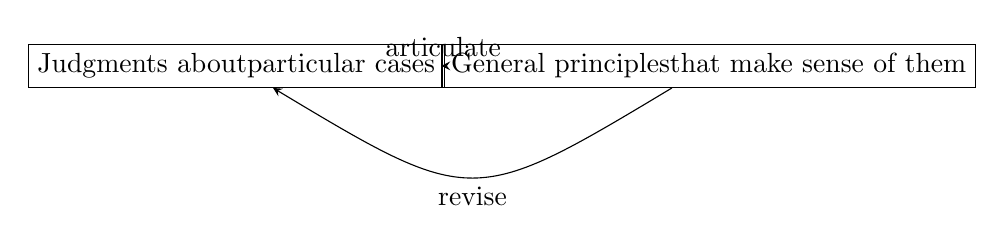
\begin{tikzpicture}[>=stealth]
\node[draw, rectangle] (A) at (0,0) {Judgments about\\particular cases};
\node[draw, rectangle] (B) at (6,0) {General principles\\that make sense of them};
\draw[->] (A) -- node[above] {articulate} (B);
\draw[->] (B) .. controls (3,-1.8) and (3,-1.8) .. node[below] {revise} (A);
\end{tikzpicture}
\end{figure}

\paragraph{Dialectical procedure.}
\begin{enumerate}
\item We begin with considered judgments about cases, stories, and examples.
\item We articulate principles that explain why we judge these cases as we do.
\item We test whether the principles and judgments fit together coherently.
\item Where the fit fails, we revise the principles, the judgments, or both.
\end{enumerate}

Sandel's crucial turn is then to Rawls. Rawls does not merely propose principles behind a veil of ignorance; he also proposes this method of justification. But Rawls restricts the method's public success to justice, not to comprehensive moral and religious questions. The reason is reasonable pluralism: conscientious people may disagree, and may continue to disagree, about the good life.

Sandel grants much of this description. The question is why justice should be exempt. Do we not also find reasonable pluralism about justice itself? Libertarians and egalitarians disagree. Citizens disagree about free speech, religious liberty, and the meaning of equality. If reasonable disagreement does not bar dialectical reasoning in the case of justice, why should it bar it in the case of the good?

\section{Respect, Moral Engagement, and the Restlessness of Reason}

This challenge to Rawls leads directly to the lecture's final worry. If justice is entangled with morality and religion, how can we sustain mutual respect in a pluralist society? Sandel's answer is that everything depends on what conception of respect we adopt.

The liberal conception is
\begin{equation}
\text{respect}_{\mathrm{liberal}}
=
\text{bracketing or abstracting from moral and religious convictions}.
\end{equation}
On this view, we respect others by not bringing their deepest convictions into political contest. We leave them aside for public purposes.

Sandel proposes a different conception:
\begin{equation}
\text{respect}_{\mathrm{engaged}}
=
\text{attending to, contesting, and learning from those convictions}.
\end{equation}
Here respect does not mean indifference. It means taking one another seriously enough to argue, to listen, to challenge, and sometimes to learn.

\subsection{Question \& Answer}

\paragraph{Question.} Does respect require setting moral convictions aside, or taking them seriously enough to engage them?

\paragraph{Answer.} Sandel argues for the second view. Engaged respect offers no guarantee of agreement, and not even a guarantee of appreciation. We may learn more about a doctrine and come to like it less. But a politics of engagement is, for Sandel, better suited to a pluralist society than a politics of abstraction.

The final conclusion is therefore not a theorem about same-sex marriage. It is a political and philosophical ideal:
\begin{equation}
\text{politics of moral engagement}
\Longrightarrow
\text{better appreciation of plural human goods}.
\end{equation}
The lecture ends by returning to the course as a whole. Philosophy estranges us from the familiar. It unsettles settled assumptions. Once the familiar turns strange, it does not become familiar again in quite the old way. This unease is not an accident. It is the tension that animates critical reflection, political improvement, and perhaps the moral life itself.

Sandel's last cadence returns to Kant. Skepticism may be a resting place for reason, but it is not a permanent dwelling place. The aim of the course has been to awaken what Kant called the restlessness of reason and to see where it leads.

\section{Summary}

The lecture moves in a deliberate arc. It begins with the narrative conception of the self and the challenge posed by segregationist appeals to history and way of life. It then tests the universalist impulse by asking what becomes of friendship if universal concern must always override particular loyalty. From there Sandel distinguishes two ways justice may be tied to the good, rejecting the relativist version and defending the non-relativist one.

The argument then enters public controversy through same-sex marriage. The class discussion generates the decisive distinctions: procreation versus union, private morality versus public recognition, neutrality versus disestablishment. Goodridge shows that once the state remains in the business of honoring marriage, it cannot avoid the question of what marriage is for. That yields the broader philosophical conclusion that reasoning about the good is unavoidable in arguments about justice.

Finally, Sandel turns to method and to politics. Reflective equilibrium shows how such reasoning proceeds without a single master principle, and the closing contrast between liberal respect and engaged respect gives the lecture its civic meaning. The course ends, not with closure, but with the claim that philosophy remains inescapable because we are always already living some answer to these questions.